\documentclass[11pt]{article}
\usepackage[margin=1in]{geometry}

\usepackage{amsmath}
\usepackage{amssymb}
\usepackage[utf8]{inputenc} 
\usepackage{graphicx} 
\usepackage{parskip} 
\usepackage{multirow} 
\usepackage{mathtools}

\DeclarePairedDelimiter\abs{\lvert}{\rvert}%
\DeclarePairedDelimiter\norm{\lVert}{\rVert}%

\makeatletter
\let\oldabs\abs
\def\abs{\@ifstar{\oldabs}{\oldabs*}}

\let\oldnorm\norm
\def\norm{\@ifstar{\oldnorm}{\oldnorm*}}
\makeatother
\usepackage{multicol} 
\usepackage[spanish,es-nodecimaldot]{babel} 
\usepackage{mathtools}
\usepackage{amsfonts}
\usepackage{float}
\usepackage{textcomp}
\usepackage{caption}
\usepackage{subfig}
\usepackage[spanish]{babel}
\usepackage{gensymb}
\def\sen{\mathop{\mbox{\normalfont sen}}\nolimits}

\usepackage{fancyhdr}
\fancyhf{}
\rfoot{\thepage}
\pagestyle{fancy}
\lhead{Nieto Castellanos Fabián}
\chead{}
\rhead{Tarea 9. Histogramas}
\begin{document}

\textbf{1)}
\begin{figure}[H]
\centering
\subfloat[Resolución en el eje $X$ para todos los eventos.]{
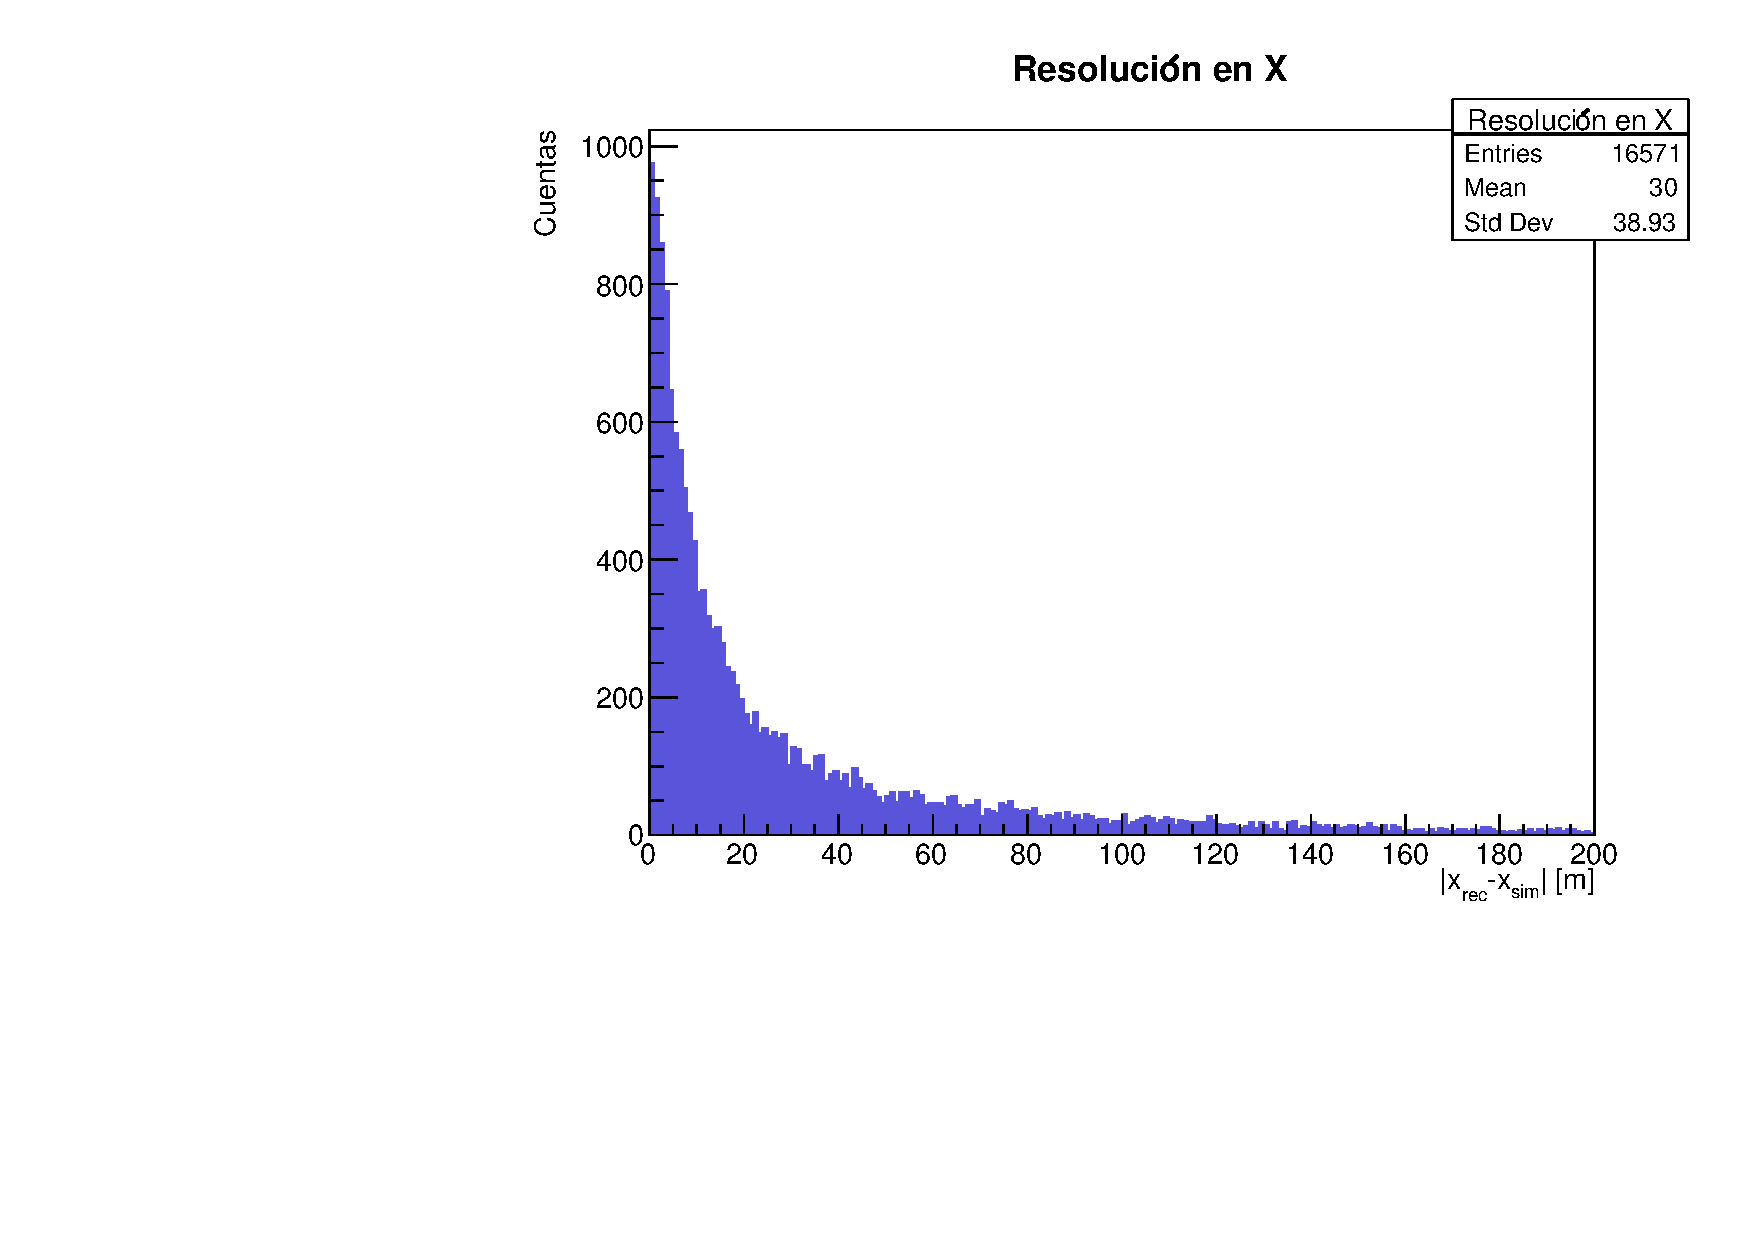
\includegraphics[width=0.8\textwidth]{../Figuras/Prob1A.pdf}}

\subfloat[Resolución en el eje $Y$ para todos los eventos.]{
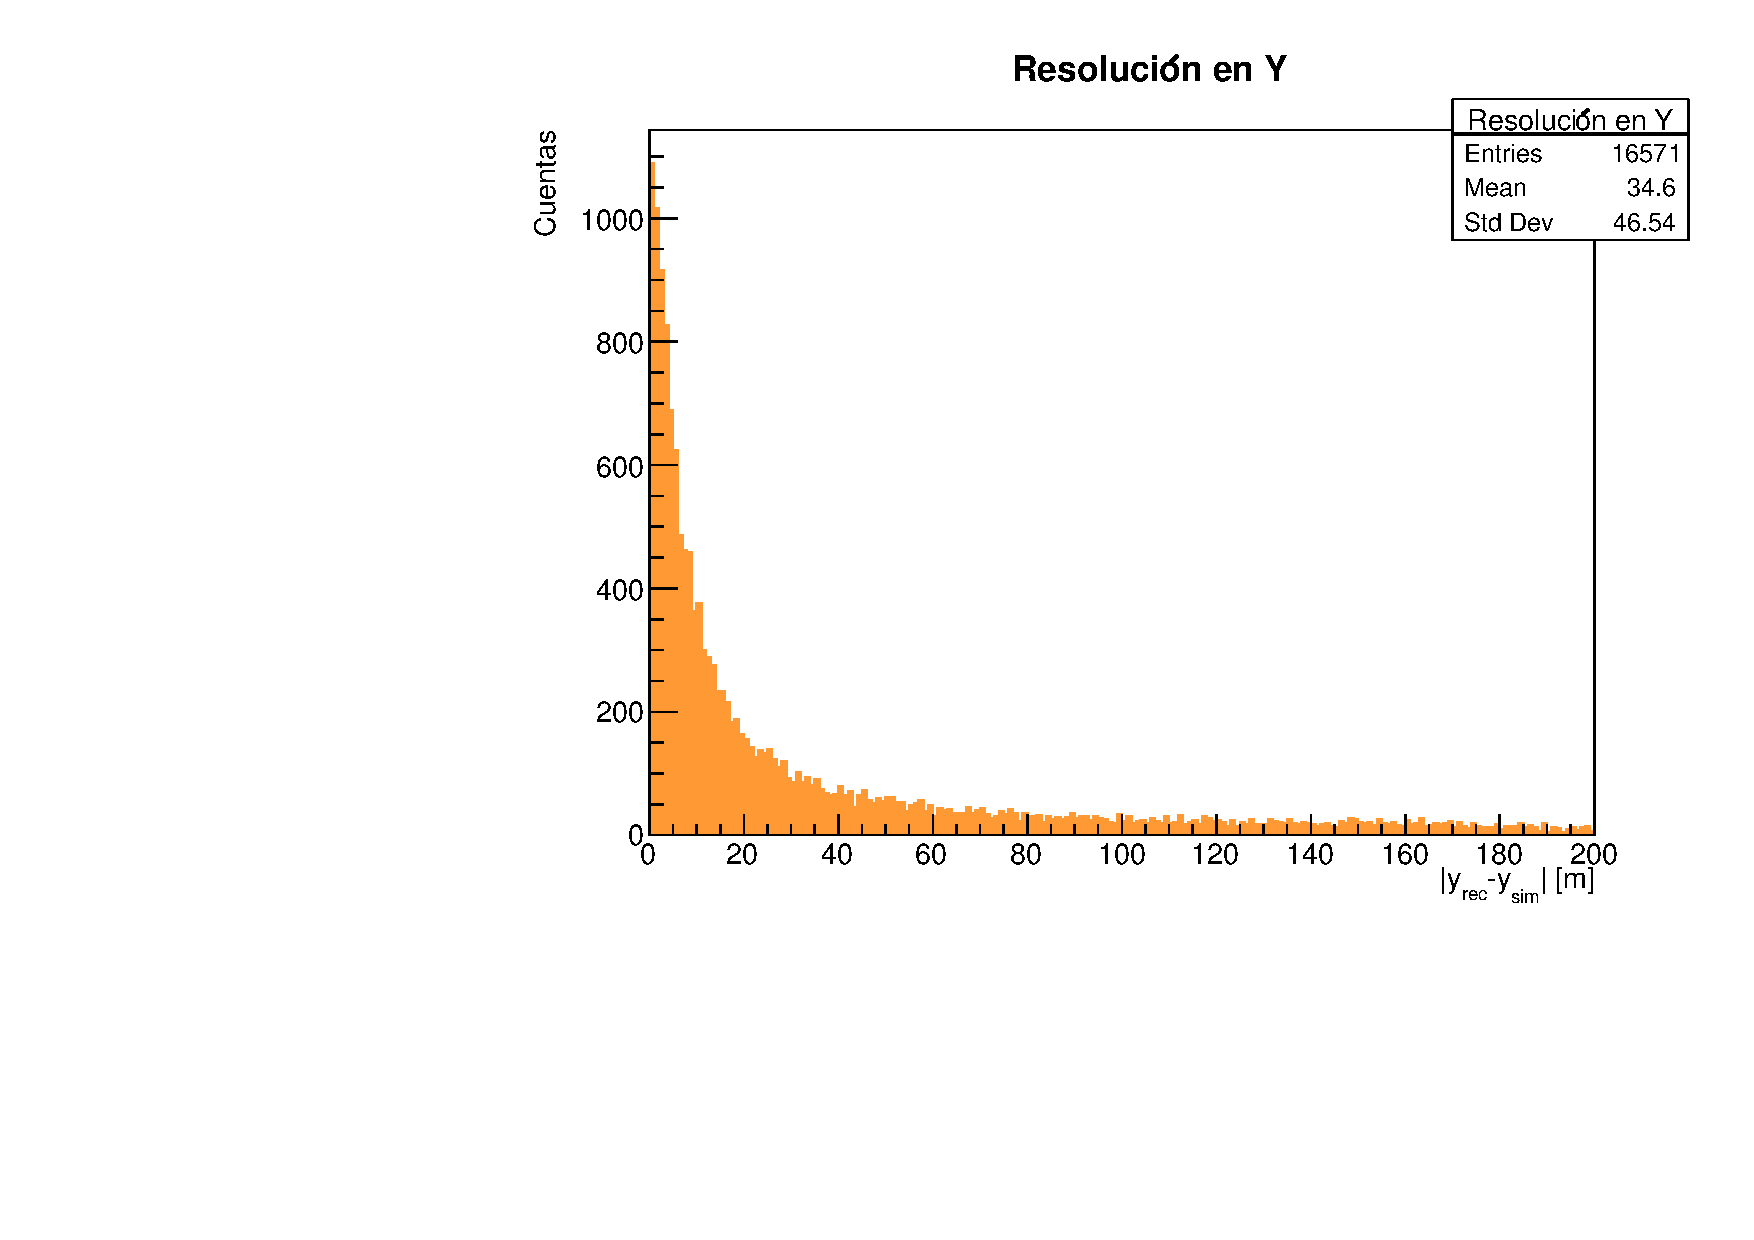
\includegraphics[width=0.8\textwidth]{../Figuras/Prob1B.pdf}}
\caption{Resolución en los ejes $X$, $Y$ tomando en cuenta todos los eventos.}
\label{fig:Prob1AB}
\end{figure}


\begin{figure}[H]
\centering
\subfloat[Resolución en el eje $X$, haciendo filtro con coreFiduScale]{
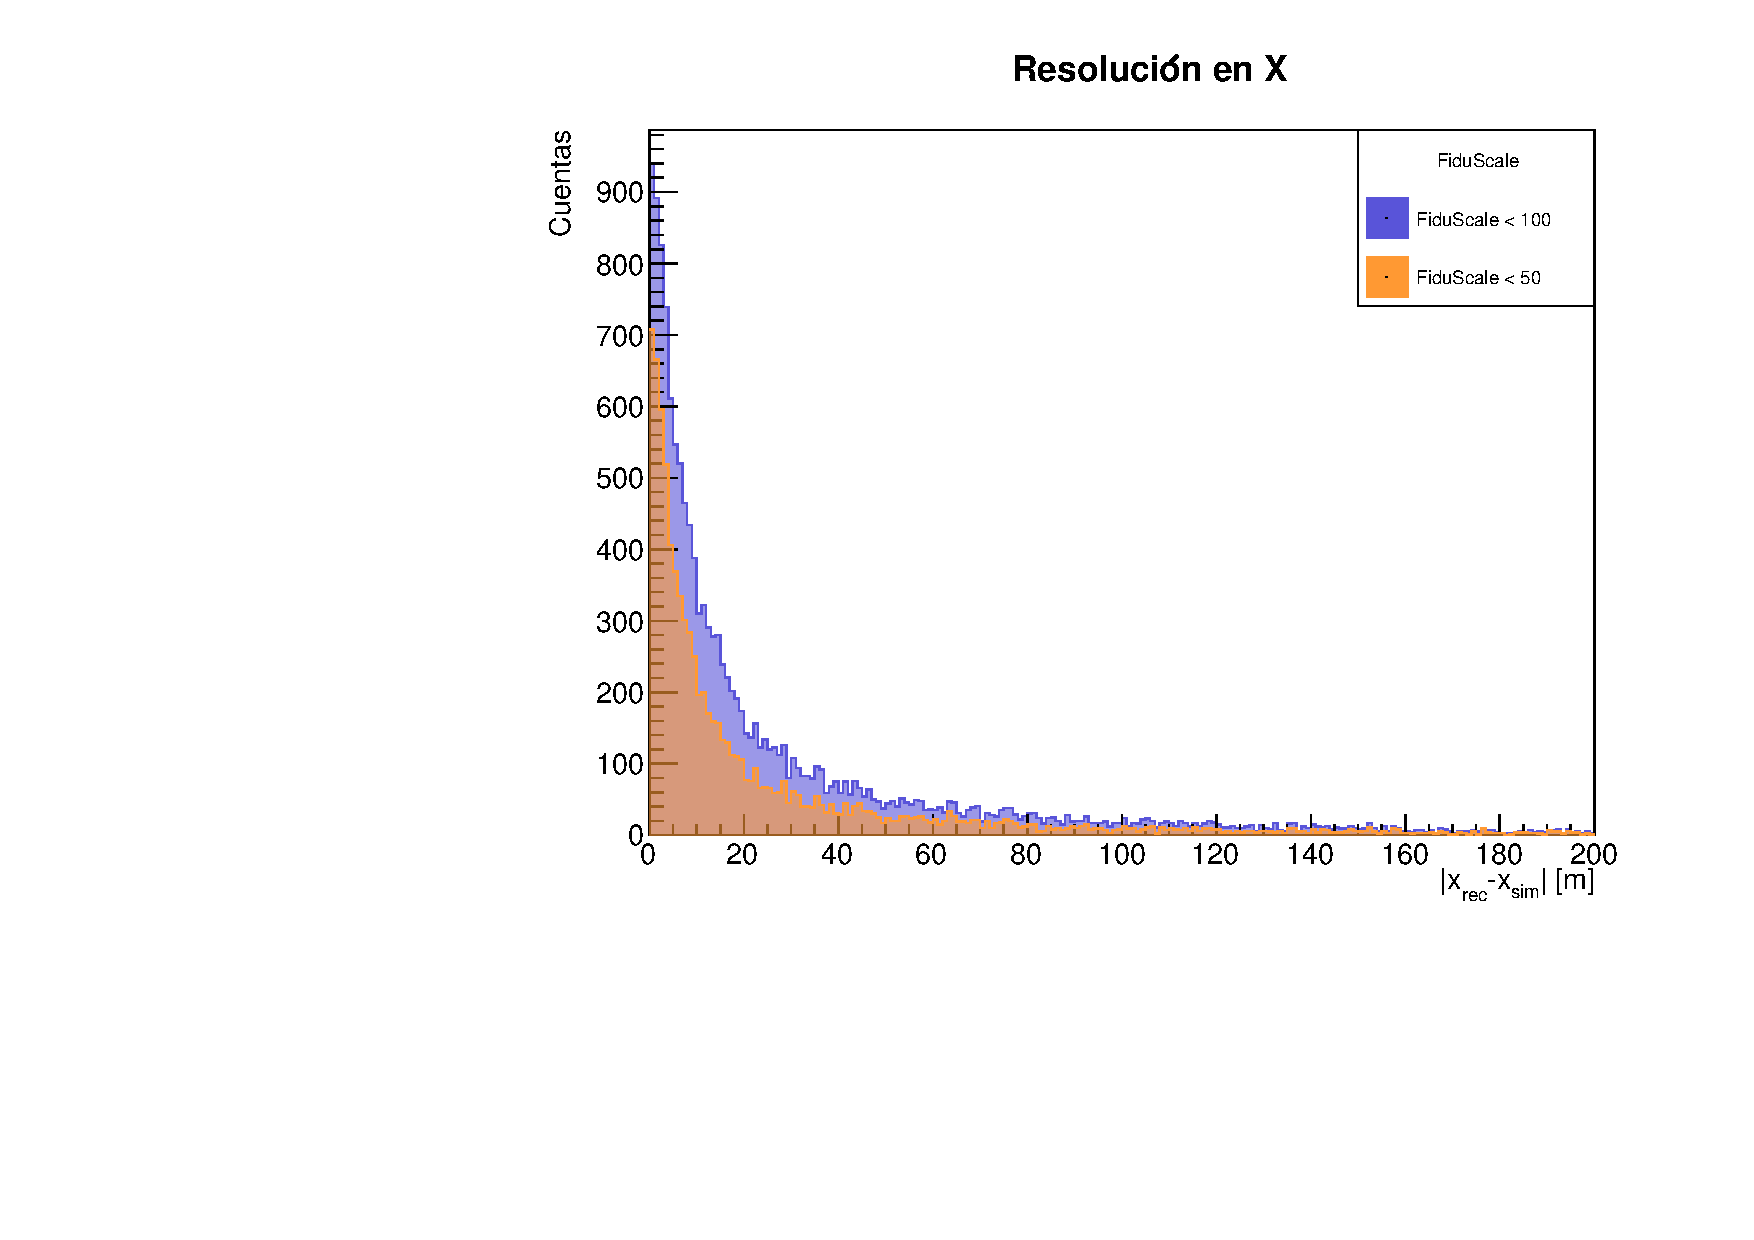
\includegraphics[width=0.8\textwidth]{../Figuras/Prob1C.pdf}}

\subfloat[Resolución en el eje $Y$, haciendo filtro con coreFiduScale]{
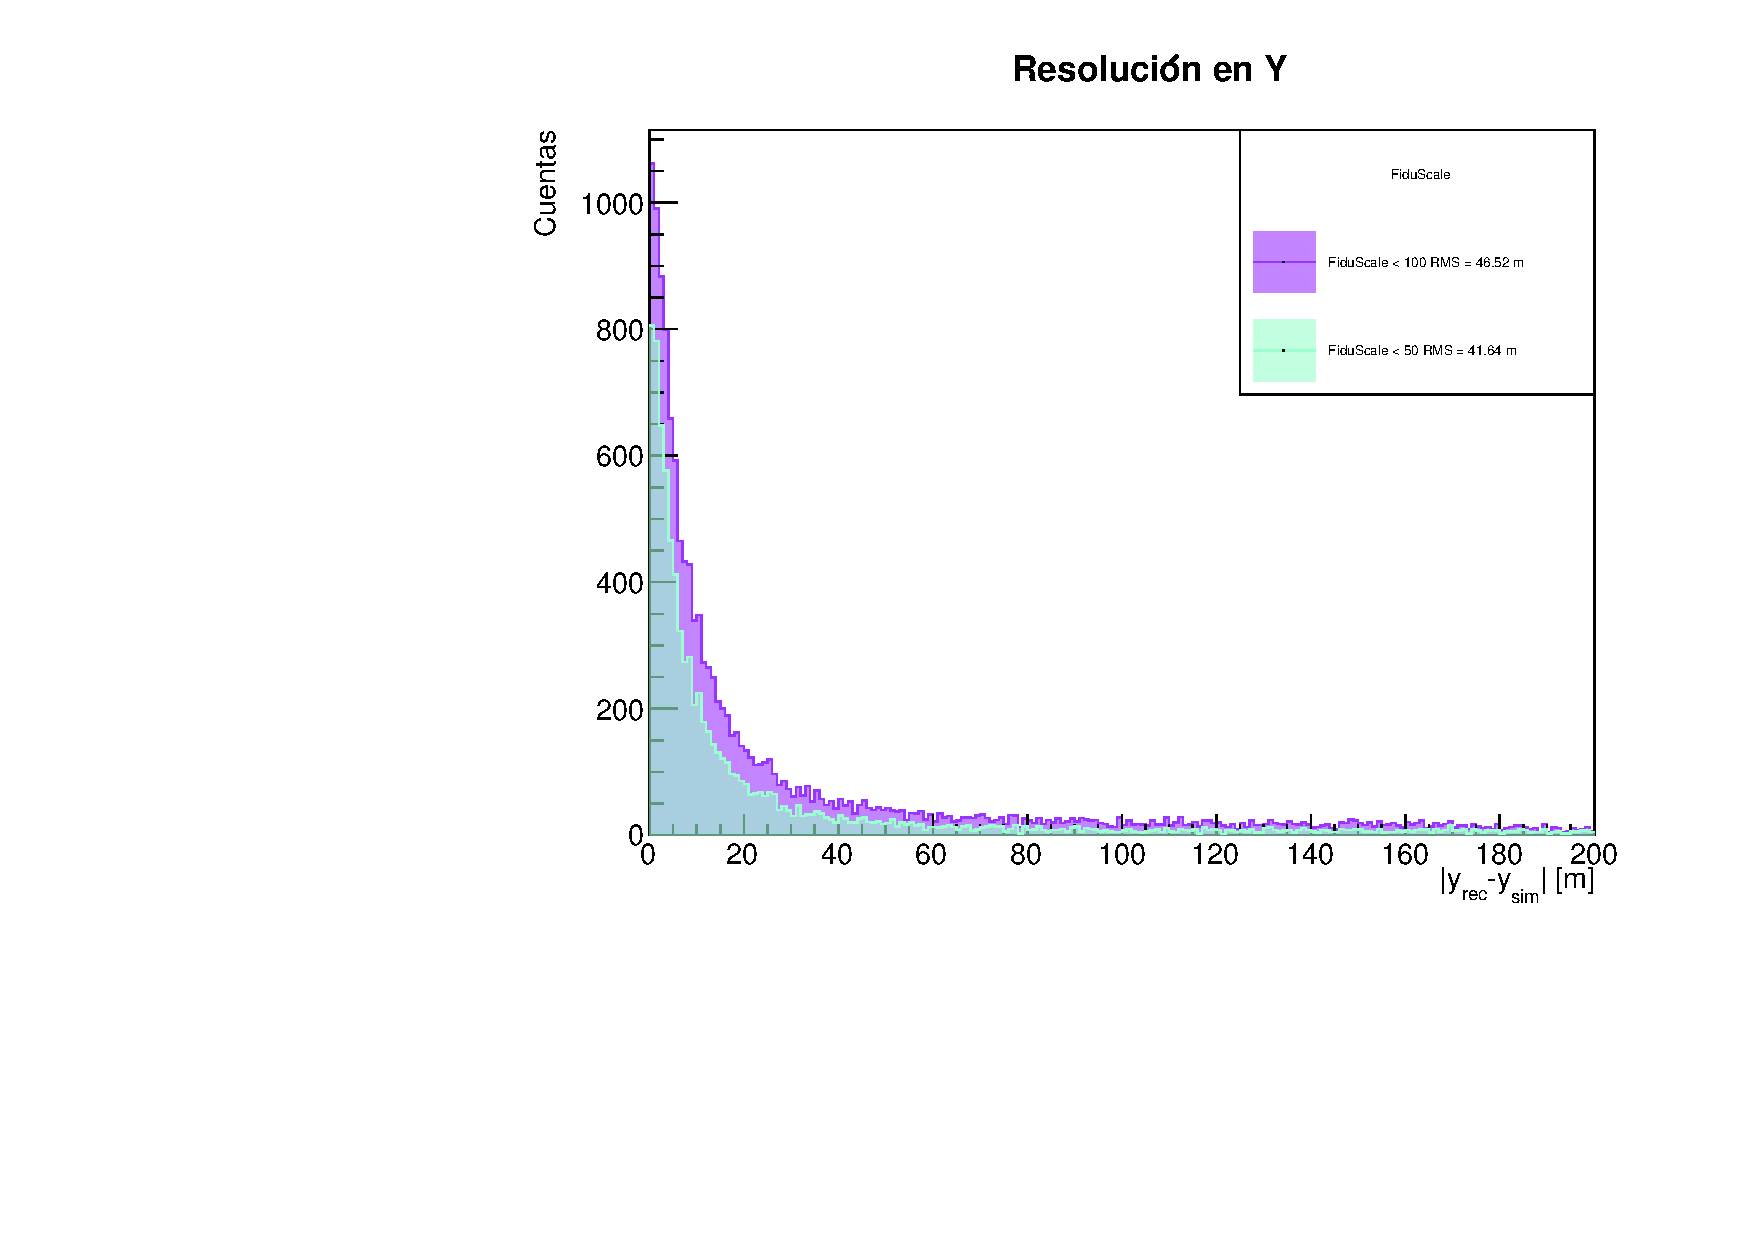
\includegraphics[width=0.8\textwidth]{../Figuras/Prob1D.pdf}}
\caption{Resolución en los ejes $X$, $Y$ haciendo un filtro con la variable coreFiduScale.}
\label{fig:Prob1CD}
\end{figure}

\pagebreak
%%%%%%%%%%%%%%%%%%%%%%%%%%%%%%%%%%%%%%%%%%%%%%%%%%%%%%
\textbf{2)}
\begin{figure}[H]
\centering
\subfloat[Resolución del ángulo cenital para eventos con más y menos de 100 hits.]{
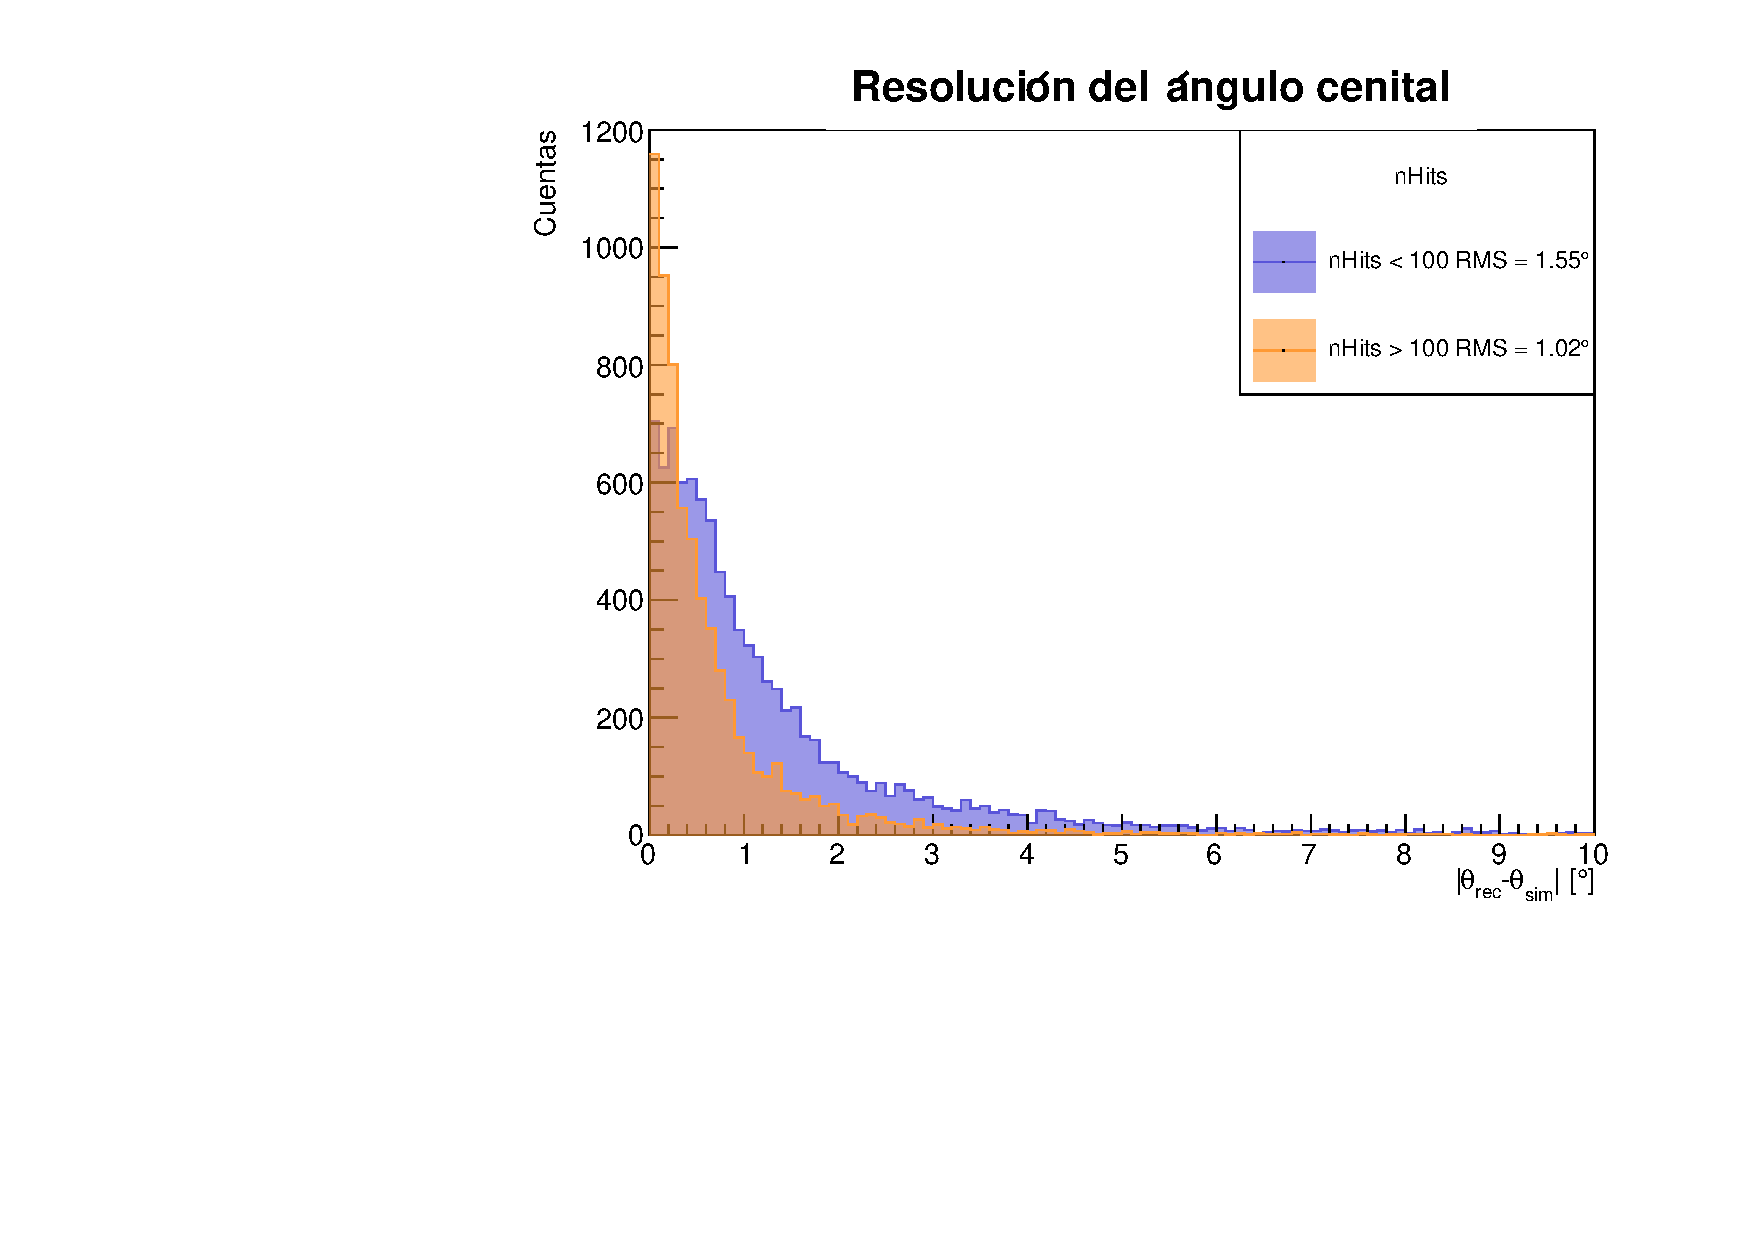
\includegraphics[width=0.78\textwidth]{../Figuras/Prob2A.pdf}}

\subfloat[Resolución del ángulo acimutal para eventos con más y menos de 100 hits.]{
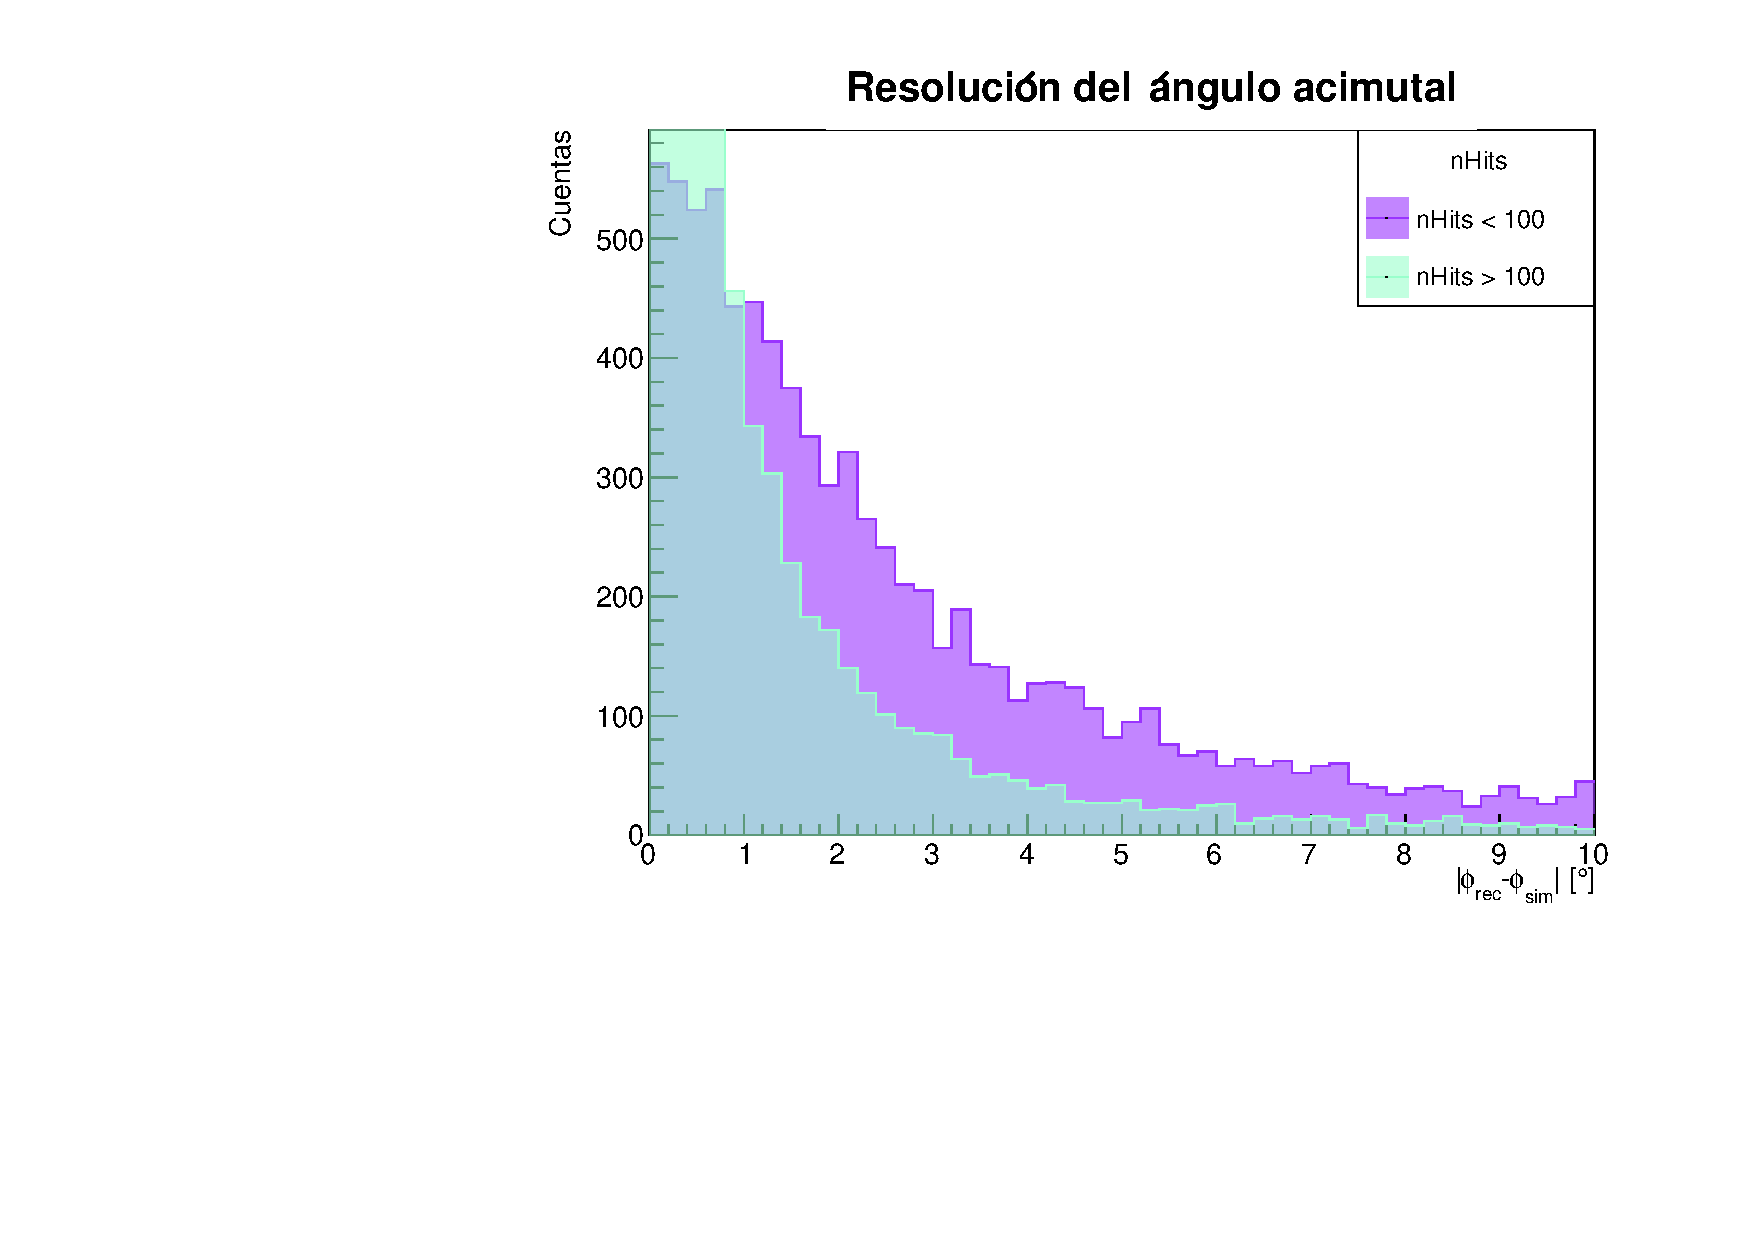
\includegraphics[width=0.78\textwidth]{../Figuras/Prob2C.pdf}}
\caption{Resolución de los ángulos cenital y acimutal tomando en cuenta el número de hits por evento.}
\label{fig:Prob2AC}
\end{figure}


\begin{figure}[H]
\centering
\subfloat[Resolución del ángulo cenital para eventos con diferente valor de coreFiduScale.]{
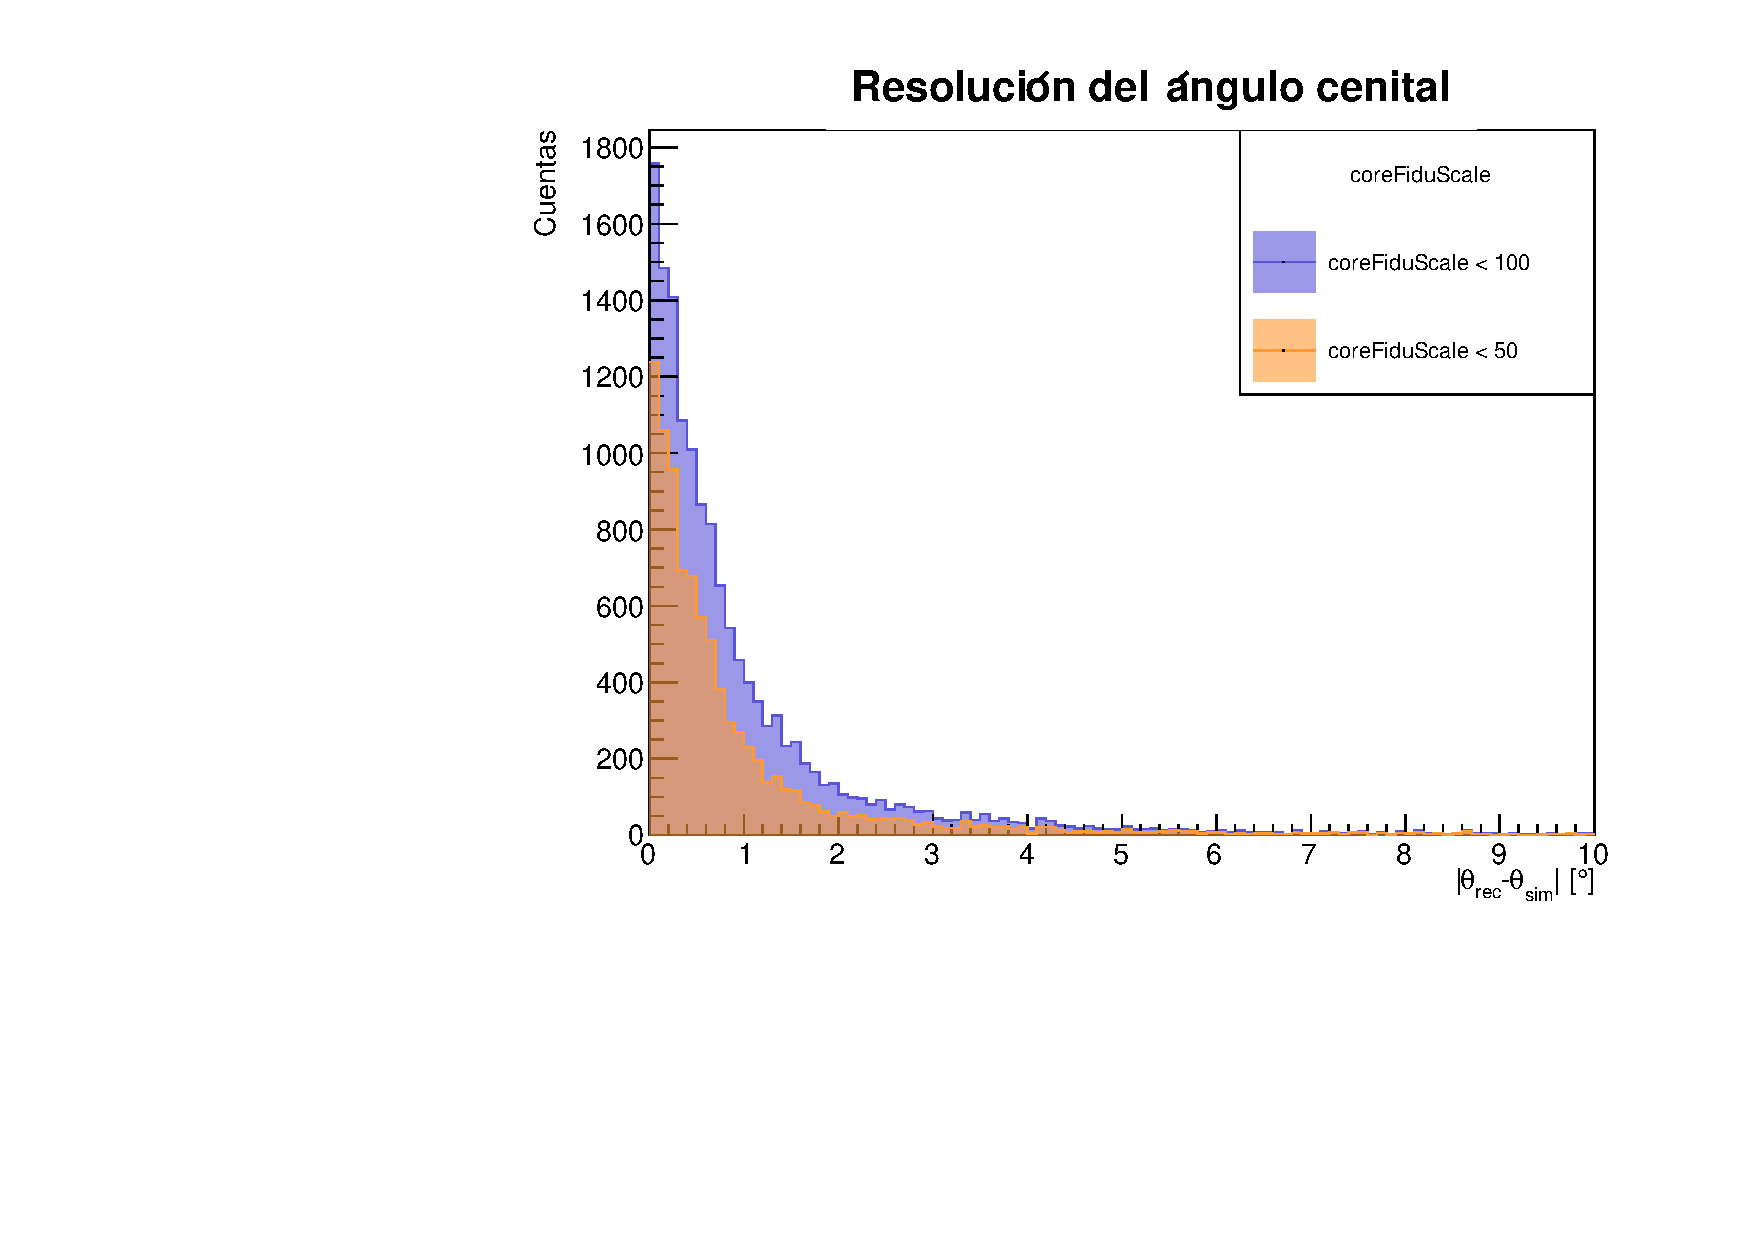
\includegraphics[width=0.78\textwidth]{../Figuras/Prob2B.pdf}}

\subfloat[Resolución del ángulo acimutal para eventos con diferente valor de coreFiduScale.]{
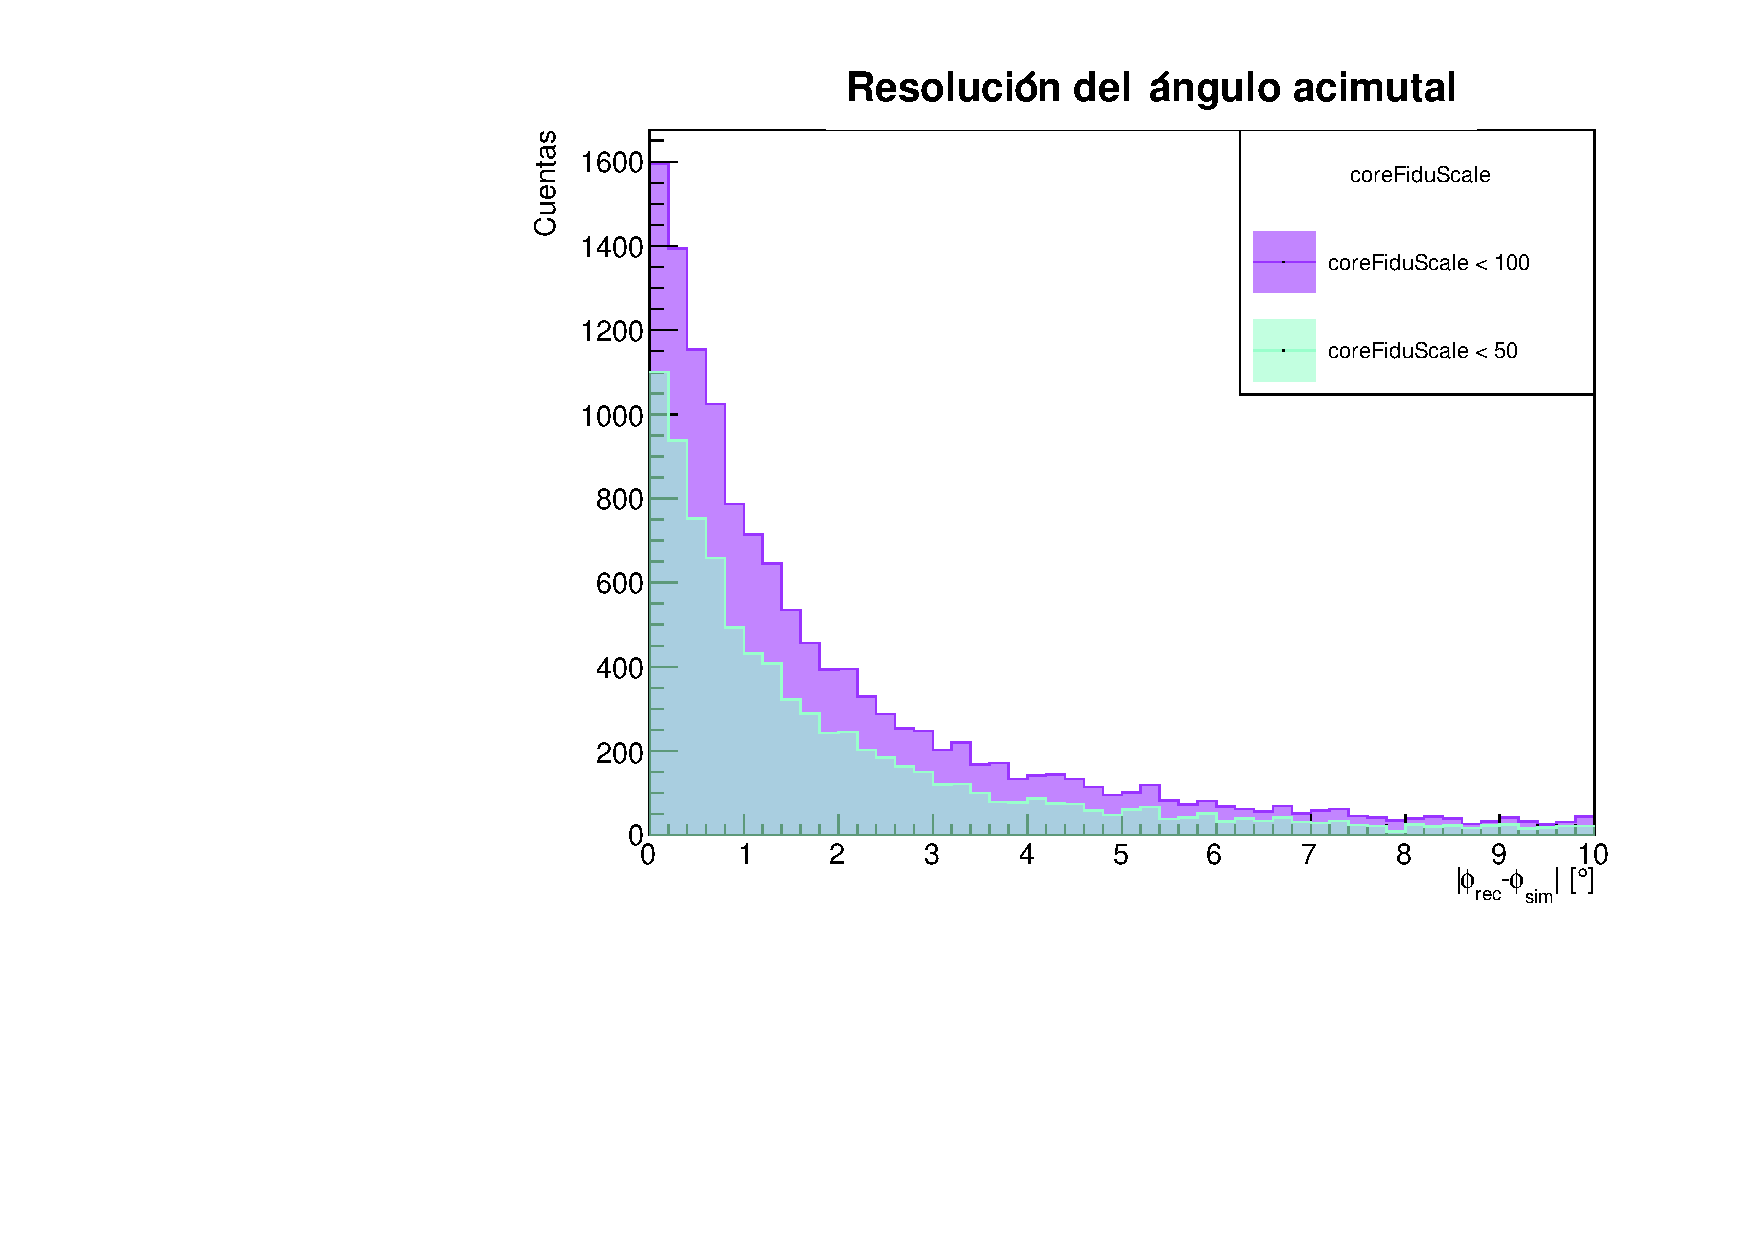
\includegraphics[width=0.78\textwidth]{../Figuras/Prob2D.pdf}}
\caption{Resolución de los ángulos cenital y acimutal tomando en cuenta la variable coreFiduScale.}
\label{fig:Prob2BD}
\end{figure}

\end{document}